\documentclass[dvipsnames,tikz]{standalone}
\usepackage{amsmath}
\usepackage{xcolor}
\usepackage{tikz}
\usetikzlibrary{calc}
\usepackage{cmbright}      % sansfont

\usepackage{ifthen}

\tikzset{main/.style={circle, color=black}}


% USE THE FOLLOWING IMAGEMAGICK CMD to convert to animated png
% magick -density 300 -delay 3 -loop 0 image.pdf -duplicate 1,-2-1 APNG:image.png

\begin{document}
	\begin{tikzpicture}[scale=0.75, main, line join=bevel]
		\draw[main] (0,0) rectangle (8,1);
		\foreach \x in {1,...,7} {
			\draw[main] (\x,0) -- (\x,1);
		}
		\draw[|-|, main, yshift=-10pt] (0,0) -- (1,0);
		\draw[main] (0.5,0) node[yshift=-2pt,below] {\tiny 4096};
	\end{tikzpicture}

	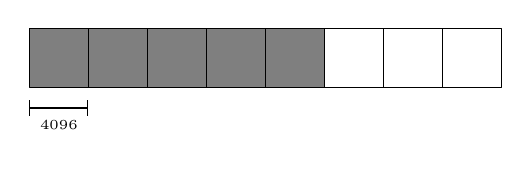
\begin{tikzpicture}[scale=0.75, main, line join=bevel]
		\fill[main, semitransparent] (0,0) rectangle (5,1);
		\draw[main] (0,0) rectangle (8,1);
		\foreach \x in {1,...,7} {
			\draw[main] (\x,0) -- (\x,1);
		}
		\draw[|-|, main, yshift=-10pt] (0,0) -- (1,0);
		\draw[main] (0.5,0) node[yshift=-2pt,below] {\tiny 4096};
	\end{tikzpicture}
\end{document}